%!TEX TS-program = xelatex
%!TEX root = ../Topo2_WS15/topologie_2.tex
\RequirePackage{fix-cm} 
\documentclass[a4paper, twoside, headsepline, index=totoc,toc=listof, fontsize=10pt, cleardoublepage=empty, headinclude, DIV=12, BCOR=5mm, titlepage,draft]{scrartcl}
\usepackage{scrtime} % KOMA, Uhrzeit ermoeglicht

\usepackage{etoolbox}
\usepackage{letltxmacro}
\usepackage{ifthen}

%--Farbdefinitionen
%-- muss vor tikz geladen werden
\usepackage[usenames, table, x11names]{xcolor}
\definecolor{dark_gray}{gray}{0.45}
\definecolor{light_gray}{gray}{0.6}
\usepackage[final]{graphicx}

%--Zum Zeichnen
%-- muss vor polyglossia bzw. babel geladen werden
\usepackage{tikz}
\usepackage{tikz-cd}
\usetikzlibrary{external}
\tikzset{>=latex}
\usetikzlibrary{shapes,arrows.meta,intersections}
\usetikzlibrary{calc,3d}
\usetikzlibrary{decorations.pathreplacing,decorations.markings, decorations.pathmorphing}
\usetikzlibrary{angles}

%-- Konfiguration von tikzexternalize
\tikzexternalize[prefix=tikz/,up to date check=diff]
\pgfkeys{/pgf/images/include external/.code=\includegraphics{#1}}
\tikzset{external/system call={xelatex \tikzexternalcheckshellescape -halt-on-error -interaction=batchmode --shell-escape -jobname "\image" "\texsource"}}


%-- tikzexternalize fuer tikzcd deaktivieren, da inkompatibel
\AtBeginEnvironment{tikzcd}{\tikzexternaldisable}
\AtEndEnvironment{tikzcd}{\tikzexternalenable}

%-- um Inkompatibilitaeten von quotes und polyglossia bzw. babel zu vermeiden
\tikzset{
  every picture/.append style={
    execute at begin picture={\shorthandoff{"}},
    execute at end picture={\shorthandon{"}}
  }
}
\usetikzlibrary{quotes}
\usepackage{pgfplots}
\usepgfplotslibrary{colormaps}
% \pgfplotsset{compat=1.12}



%-- Mathesymbole etc.
\usepackage{mathtools} % beinhaltet amsmath
\mathtoolsset{showonlyrefs, centercolon,showmanualtags}
\newtagform{brackets}[\textbf]{[}{]}
\usetagform{brackets}
\usepackage{fix-cm}
% \usepackage{wasysym} % zusätzliche Symbole
\usepackage{amssymb} % zusätzliche Symbole
% \usepackage{stmaryrd} % für Blitz
\usepackage{nicefrac} % schräge Brüche
\usepackage{faktor}
\newcommand{\Faktor}[1]{\faktor[\textstyle]{#1}}
\usepackage{xfrac}
\usepackage{cancel}
\usepackage{mathdots} % Verbesserung von Punkten wie zB \ldots
\usepackage[bb=px]{mathalfa}

%-- einzelne Symbole aus dem mathx-package
% \DeclareFontFamily{U}{mathx}{\hyphenchar\font45}
% \DeclareFontShape{U}{mathx}{m}{n}{<-> mathx10}{}
% \DeclareSymbolFont{mathx}{U}{mathx}{m}{n}
% \DeclareMathSymbol{\bigplus}{1}{mathx}{"90}

%-- 
\usepackage{silence}
\WarningFilter{latexfont}{Size substitutions with differences}
\WarningFilter{latexfont}{Font shape `U/bbold/m/n' in size}

\DeclareSymbolFont{bbold}{U}{bbold}{m}{n}
\DeclareSymbolFontAlphabet{\mathbbold}{bbold}
\newcommand{\ind}{\mathbbold{1}} % charakteristische-Funktion-Eins

\def\mathul#1#2{\color{#1}\underline{{\color{black}#2}}\color{black}} %farbiges Untersteichen im Mathe-Modus
\renewcommand{\le}{\leqslant}
\renewcommand{\ge}{\geqslant}

%-- Underbrace als Befehl in LaTeX-Syntax (und ohne Spacingprobleme mit nachfolgenden Operatoren...)
\newcommand{\Underbrace}[2]{{\underbrace{#1}_{#2}}}
\newcommand{\Underbracket}[2]{{\underbracket[0.7pt][2pt]{#1}_{#2}}}

%-- Alles was mit Schrift und XeTeX zu tun hat
\usepackage{palatino}
\usepackage[euler-digits]{eulervm}
\usepackage[no-math]{fontspec}
\usepackage{polyglossia} % moderner babel-ersatz
\setmainlanguage[spelling=new,babelshorthands=true]{german}
\shorthandoff{"}
\setotherlanguage{english}
\defaultfontfeatures{Mapping=tex-text, WordSpace={1.2}, Ligatures={Required,Common,Contextual}} %

%-- Alle hier aufgeführten Schriftarten sind in jeder TeXlive-Installation vorhanden!!
%-- Hauptschriftart festlegen
% \setmainfont{texgyrepagella}[Extension=.otf,UprightFont=*-regular,BoldFont=*-bold,ItalicFont=*-italic,BoldItalicFont=*-bolditalic,ItalicFeatures={Style=Historic}]
\setmainfont{TeXGyrePagellaX}[Extension=.otf,UprightFont=*-Regular,BoldFont=*-Bold,ItalicFont=*-Italic,BoldItalicFont=*-BoldItalic,ItalicFeatures={Style=Historic},Ligatures={Required,Common,Contextual,Historic}]
% \setmainfont[BoldFont={* Bold}, ItalicFont={* Light Italic},SmallCapsFont={Linux Libertine O}, SmallCapsFeatures={Letters=SmallCaps}]{Source Sans Pro}


%-- Serifenlose Schriftart festlegen
% \setsansfont{Roboto}[Scale=MatchUppercase,Extension=.ttf,UprightFont=*-Regular,BoldFont=*-Bold,ItalicFont=*-RegularItalic,BoldItalicFont=*-MediumItalic]
% \setsansfont{RobotoSlab}[Scale=MatchUppercase,Extension=.ttf,UprightFont=*-Regular,BoldFont=*-Bold,ItalicFont=*-Thin,SmallCapsFont=*-Regular]
% \setsansfont{FiraSans}[Scale=MatchUppercase,Extension=.otf, UprightFont=*-Regular, BoldFont=*-SemiBold, ItalicFont=*-RegularItalic, BoldItalicFont=*-MediumItalic]
% \setsansfont{SourceSansPro}[Scale=MatchUppercase,Extension=.otf,UprightFont=*-Regular,BoldFont=*-Semibold,ItalicFont=*-LightIt,BoldItalicFont=*-SemiboldIt]
% \setsansfont{texgyreadventor}[Scale=MatchUppercase, Extension=.otf, UprightFont=*-regular, BoldFont=*-bold, ItalicFont=*-italic,BoldItalicFont=*-bolditalic]
% \setsansfont{Kurier}[Scale=MatchUppercase, Extension=.otf, UprightFont=*Medium-Regular, BoldFont=*Heavy-Regular, ItalicFont=*Medium-Italic,BoldItalicFont=*Heavy-Italic]
% \setsansfont{Iwona}[Scale=MatchUppercase, Extension=.otf, UprightFont=*Medium-Regular, BoldFont=*Heavy-Regular, ItalicFont=*Medium-Italic,BoldItalicFont=*Heavy-Italic]
% \setsansfont{LinBiolinum}[Scale=MatchUppercase, Extension=.otf, UprightFont=*_R, BoldFont=*_RB, ItalicFont=*_RI,BoldItalicFont=*_RBO]
% \setsansfont{texgyrebonum}[Scale=MatchUppercase,Extension=.otf, UprightFont=*-regular, BoldFont=*-bold, ItalicFont=*-italic, BoldItalicFont=*-bolditalic]
\setsansfont{texgyreadventor}[Scale=MatchUppercase,Extension=.otf, UprightFont=*-regular, BoldFont=*-bold, ItalicFont=*-italic, BoldItalicFont=*-bolditalic]



% \newfontfamily{\geometric}{texgyreheros}[Scale=MatchLowercase, Extension=.otf, UprightFont=*-regular, BoldFont=*-bold, ItalicFont=*-italic]
% \addtokomafont{disposition}{\geometric}
\setmonofont{SourceCodePro}[Scale=0.9,Extension=.otf,UprightFont=*-Regular, BoldFont=*-Semibold, ItalicFont=*-Light]
\usepackage{xltxtra}
\usepackage{fontawesome}
\usepackage[final]{microtype}


\usepackage[draft=false]{scrlayer-scrpage} % wie fancyhdr, nur optimiert auf KOMA-Skript, leicht andere Syntax

\flushbottom


%--Mixed
\usepackage[shortlabels,inline]{enumitem}
\setlist[itemize,1]{label=\faCaretRight}
\setlist[enumerate]{font=\bfseries}
\setlist[description]{font=\normalfont\bfseries}
\usepackage[german=quotes]{csquotes}
\usepackage{makeidx}
\usepackage{wrapfig}
\usepackage{float}
\usepackage[margin=10pt, font=small, labelfont={sf, bf}, format=plain, indention=1em]{caption}
\captionsetup[wrapfigure]{name=Abb. }
\usepackage{stackrel}


%--Unterstreichung
\usepackage[normalem]{ulem}
\setlength{\ULdepth}{1.8pt}

%--Indexverarbeitung
\newcommand{\bet}[1]{\emph{#1}}
\newcommand{\Index}[1]{\bet{#1}\index{#1}}
\makeindex
\setindexpreamble{{\noindent\sffamily\small Die \emph{Seitenzahlen} sind mit Hyperlinks versehen und somit anklickbar}  \par \bigskip}
\renewcommand{\indexpagestyle}{scrheadings}


%--Marginnote & todonotes
\deffootnote[1.5em]{1.5em}{1.5em}{\textsuperscript{\thefootnotemark}\ }
\usepackage[fulladjust]{marginnote}
\renewcommand*{\marginfont}{\color{dark_gray} \itshape \footnotesize}
\usepackage[textsize=small]{todonotes}
\usepackage{ragged2e}
\renewcommand*{\raggedleftmarginnote}{\RaggedLeft}
\renewcommand*{\raggedrightmarginnote}{\RaggedRight}

%--Todonotes mit tikz/externalize kompatibel machen
\LetLtxMacro{\oldtodo}{\todo}
\renewcommand{\todo}[2][]{\tikzexternaldisable\oldtodo[#1]{#2}\tikzexternalenable}
\LetLtxMacro{\oldmissingfigure}{\missingfigure}
\renewcommand{\missingfigure}[2][]{\tikzexternaldisable\oldmissingfigure[{#1}]{#2}\tikzexternalenable}

%--Konfiguration von Hyperref pdfstartview=FitH, 
\usepackage[hidelinks, pdfpagelabels,  bookmarksopen=true, bookmarksnumbered=true, linkcolor=black, urlcolor=SkyBlue2, plainpages=false,pagebackref, citecolor=black, hypertexnames=true, pdfauthor={Jannes Bantje}, pdfborderstyle={/S/U}, linkbordercolor=SkyBlue2, colorlinks=false,final]{hyperref}


\newcommand{\appendLink}[1]{#1\,\faExternalLink}
\newcommand{\hrefsym}[2]{\href{#1}{\texttt{\appendLink{#2}}}}
\newcommand{\hrefsymmail}[2]{\href{#1}{\texttt{\faEnvelopeO\,#2}}}
\renewcommand{\url}[1]{\hrefsym{#1}{\nolinkurl{#1}}}



% -- QR-Codes
\usepackage{qrcode} %-- hinter hyperref laden!

%--Römische Zahlen
\newcommand{\RM}[1]{\MakeUppercase{\romannumeral #1{}}}

%%--Abkürzungen etc.
\newcommand{\light}{\text{\Large $\lightning$}}

%-- Definitionen von weiteren Mathe-Befehlen

\DeclareMathOperator{\im}{im} %Bild
\DeclareMathOperator{\id}{id} %identische Abbildung
\DeclareMathOperator{\conj}{conj} %Konjugation
\DeclareMathOperator{\sgn}{sgn} %Signum
\DeclareMathOperator{\End}{End} %Endomorphismen
\DeclareMathOperator{\Hom}{Hom} %Homomorphismen
\DeclareMathOperator{\Iso}{Iso} %Isomorphismen
\DeclareMathOperator{\Span}{span} %Span

\DeclareMathOperator{\grad}{grad} %Gradient
\DeclareMathOperator{\dive}{div} %Gradient
\DeclareMathOperator{\rot}{rot} %Rotation


\DeclareMathOperator{\Char}{char} %Charakteristik
\DeclareMathOperator{\Aut}{Aut} %Automorphismen

% -- Zum Finetuning von Befehlen
\makeatletter
\newcommand{\raisemath}[1]{\mathpalette{\raisem@th{#1}}}
\newcommand{\raisem@th}[3]{\raisebox{#1}{$#2#3$}}
\makeatother

\newcommand{\sing}{{\raisemath{1.1pt}{\scriptscriptstyle\mathrm{sing}}}}
\newcommand{\pt}{\mathrm{pt}}
\newcommand{\op}{\mathrm{op}}
\DeclareMathOperator{\Sp}{Sp}
\DeclareMathOperator{\Keg}{Keg}
\newcommand{\slashedi}{i\hspace{-3.5pt}/}
\newcommand{\cupp}{\smallsmile}
\newcommand{\capp}{\smallfrown}
\DeclareMathOperator*{\colim}{colim}


\newcommand{\D}{\ensuremath{\mathrm{D}\mkern-1.5mu}}
\newcommand{\mathd}{\ensuremath{\mathrm{d}\mkern-1.0mu}}
\newcommand{\Tmap}{\ensuremath{\mathrm{T}\mkern-0.85mu}}
\newcommand{\opL}{\ensuremath{\mathrm{L}\mkern-0.6mu}}


\DeclareMathOperator{\supp}{supp} %Träger


% -- Befehle für FunkAna und Operatoralgebren
\newcommand{\tr}{\mathrm{tr}}
\newcommand{\w}{\mathrm{w}}
\newcommand{\sa}{\mathrm{sa}}
\newcommand{\so}{\mathrm{s.o.}}
\newcommand{\weakT}[1]{\ensuremath{\mathcal{T}_{#1}^{\mkern+1.0mu\text{\raisebox{0.4ex}{$\mathrm{w}$}}}}}
\newcommand{\weakTstar}[1]{\ensuremath{\mathcal{T}_{#1}^{\mkern+1.0mu\text{\raisebox{0.4ex}{$\mathrm{w}$}}^*}}}
\newcommand{\finSub}{\subset\mkern-0.7mu \subset}
\DeclareMathOperator{\Inv}{Inv}
\DeclareMathOperator{\dist}{dist}
\newcommand{\simm}{{\hspace{-1.6pt}\raisemath{0.5pt}{\sim}}}
\DeclareMathOperator{\ev}{ev}
\DeclareMathOperator{\Alg}{Alg}


% -- Kategorien
\newcommand{\TOP}{\textsc{Top}}
\newcommand{\HTOP}{\textsc{HTop}}
\newcommand{\VR}{\textsc{VR}}
\newcommand{\MOD}{\textsc{Mod}}
\newcommand{\MONOIDE}{\textsc{Monoide}}
\newcommand{\MENGEN}{\textsc{Mengen}}
\newcommand{\MAN}{\textsc{Man}}
\newcommand{\GRUPPEN}{\textsc{Gruppen}}
\newcommand{\ABELGRUPPEN}{\textsc{Abel.Gruppen}}
\newcommand{\KAT}{\textsc{Kat}}
\newcommand{\FUN}{\textsc{Fun}}
\newcommand{\SIMP}{\textsc{Simp}}
\newcommand{\VEKT}{\textsc{Vekt}}

\DeclareMathOperator{\cell}{cell}
\DeclarePairedDelimiter{\homologieklasse}{\llbracket}{\rrbracket}
\newcommand{\rand}[1]{\ensuremath{\partial^{\scriptscriptstyle #1}}}


% -- theorem packages
\usepackage{amsthm}
\usepackage{thmtools,thm-restate}
\renewcommand{\listtheoremname}{Übersicht aller Aussagen}

% -- Theoreme als PDF-Lesezeichen
\usepackage{bookmark}
\bookmarksetup{open,numbered}
\makeatletter
\newcommand*{\theorembookmark}{%
  \bookmark[
    dest=\@currentHref,
    rellevel=1,
    keeplevel,
  ]{%
    \thmt@thmname\space\csname the\thmt@envname\endcsname
    \ifx\thmt@shortoptarg\@empty
    \else
      \space(\thmt@shortoptarg)%
    \fi
  }%
}   
\makeatother

% -- Definition der einzelnen Umgebungen
\declaretheoremstyle[%
	headfont=\sffamily\bfseries,
	notefont=\normalfont\sffamily\scshape,
	bodyfont=\normalfont,
	headformat=\NUMBER\ \NAME\NOTE,
	headpunct=.,
	postheadspace=1em,
	spaceabove=15pt,spacebelow=10pt,
	postheadhook=\theorembookmark]%
{mainstyle}
\declaretheoremstyle[%
	headfont=\sffamily\bfseries,
	notefont=\normalfont\sffamily\scshape,
	bodyfont=\normalfont,
	headformat=\NUMBER\NAME\NOTE,
	headpunct=.,
	postheadspace=1em,
	spaceabove=15pt,spacebelow=10pt,
	postheadhook=\theorembookmark]%
{mainstyle_unnumbered}
\declaretheoremstyle[%
	headfont=\sffamily\bfseries,
	notefont=\normalfont\sffamily\scshape,
	bodyfont=\normalfont,
	headformat=swapnumber,
	headpunct=.,
	postheadspace=1em,
	spaceabove=15pt,spacebelow=10pt,
	postheadhook=\theorembookmark,
	qed=\qedsymbol]%
{mainstyleB}
\declaretheorem[name=Definition,parent=section,style=mainstyle]{definition}
\declaretheorem[name=Definition,numbered=no,style=mainstyle_unnumbered]{definition*}
\declaretheorem[name=Theorem,sharenumber=definition,style=mainstyle]{theorem}
\declaretheorem[name=Theorem,numbered=no,style=mainstyle_unnumbered]{theorem*}
\declaretheorem[name=Proposition,sharenumber=definition,style=mainstyle]{proposition}
\declaretheorem[name=Lemma,sharenumber=definition,style=mainstyle]{lemma}
\declaretheorem[name=Satz,sharenumber=definition,style=mainstyle]{satz}
\declaretheorem[name=Korollar,sharenumber=definition,style=mainstyle]{korollar}
\declaretheorem[name=Korollar,sharenumber=definition,style=mainstyleB]{korollarB}
\declaretheorem[name=Frage,numbered=no,style=mainstyle_unnumbered]{frage}
\declaretheorem[name=Erinnerung,sharenumber=definition,style=mainstyle]{erinnerungA}


% -- Beweise
\declaretheoremstyle[headfont=\bfseries\scshape,bodyfont=\normalfont,headpunct=:,postheadspace=1em,spacebelow=12pt,spaceabove=2pt,qed=\qedsymbol]{beweise}
\declaretheoremstyle[headfont=\sffamily\bfseries,bodyfont=\normalfont,headpunct=:,postheadspace=1em,spacebelow=10pt,spaceabove=10pt]{bemerkungen}
\declaretheorem[name=Beweis,numbered=no,style=beweise]{beweis}
\declaretheorem[name=Bemerkung,sharenumber=definition,style=mainstyle]{bemerkung}
\declaretheorem[name=Beispiel,sharenumber=definition,style=mainstyle]{beispiel}
\declaretheorem[name=Übung,numbered=no,style=bemerkungen]{uebung}
\declaretheorem[name=Erinnerung,numbered=no,style=bemerkungen]{erinnerung}


%--Skalarprodukt
\DeclarePairedDelimiterX\sprod[2]{\langle}{\rangle}{#1\,\delimsize\vert\,#2}
\DeclarePairedDelimiterX\skal[2]{\langle}{\rangle}{#1\,,\,#2}

%--Betrag, Gaußklammer
\DeclarePairedDelimiter{\abs}{\lvert}{\rvert}
\DeclarePairedDelimiter{\floor}{\lfloor}{\rfloor}
\DeclarePairedDelimiter{\ceil}{\lceil}{\rceil}

%--Norm
\DeclarePairedDelimiter\norm{\Vert}{\Vert}


%--Umklammern
\DeclarePairedDelimiter\enbrace{(}{)}
\DeclarePairedDelimiter\benbrace{[}{]}
\DeclarePairedDelimiter\lenbrace{<}{>}
\newcommand{\ssbrace}[1]{{\scriptscriptstyle\enbrace{#1}}}

%--Mengen
\newcommand\SetSymbol[1][]{\nonscript\:#1\vert\allowbreak\nonscript\:\mathopen{}}
\providecommand\given{} % to make it exist
\DeclarePairedDelimiterX\set[1]\{\}{\renewcommand\given{\SetSymbol[\delimsize]}#1}

%--Abbildungsdefinition
\newcommand{\mapdef}[5]{%
	\[
		\begin{array}{rcl}
			\textstyle #1 &\xrightarrow{\minwidthbox{#5}{2em}} & \textstyle #2 \\[0.5ex]
			\textstyle #3 &\xmapsto{\minwidthbox{\mbox{ }}{2em}} & \textstyle #4
		\end{array}
	\]
}

%--modifiziertes Stackrel
\newcommand{\StackText}[2]{\stackrel{\mbox{\scriptsize #1}}{#2}}

%--Befehl für eine Box mit Mindestweite
\DeclareRobustCommand{\minwidthbox}[2]{%
  \ifmmode
    \expandafter\mathmakebox
  \else
    \expandafter\makebox
  \fi
  [\ifdim#2<\width\width\else#2\fi]{#1}%
}

%--Befehl zum Einkreisen
\newcommand*\circled[1]{\tikzexternaldisable\tikz[baseline=(char.base)]{\node[shape=circle,draw,inner sep=2pt] (char) {#1};}\tikzexternalenable}


%--Differential
\newcommand{\diff}[2]{\ensuremath{\frac{{\partial #1}}{{\partial #2}} }}
\newcommand{\diffd}[2]{\ensuremath{\frac{\mathd #1}{\mathd #2} }}

%--Inhaltsverzeichnis
\usepackage[tocindentauto]{tocstyle}
\usetocstyle{KOMAlike}	
\shorthandon{"}
		
%--Punkte (als letztes laden)
\usepackage{ellipsis}

\newcommand{\fach}{Topologie \RM{2}.}
\newcommand{\semester}{WiSe 2015}
\newcommand{\homepage}{https://wwwmath.uni-muenster.de/das/ist/kein/echter/Link.html}

\newcommand{\prof}{Prof.\ Dr.\ Arthur Bartels}
% \publishers{\scalebox{14}{$K$}}
\providecommand{\verfasser}{Jannes Bantje}

%--Konfiguration von scrheadings
\setheadsepline{1pt}[\color{light_gray}]
\pagestyle{scrheadings}
%\fancyhf[H, F]{}
\clearscrheadfoot

\providecommand{\shortFach}{\fach}
\lehead{ 
\includegraphics[height=0.5 cm,keepaspectratio]{../!config/Bilder/Logo_WWU_Muenster_light_gray.pdf}}
\rehead{\rule{0cm}{0.5cm}\footnotesize \sffamily \color{light_gray} \verfasser -- Mitschrift \shortFach}
\lohead{\rule{0cm}{0.5cm} \footnotesize \sffamily \color{light_gray} Stand: \today \; \thistime[:]}
\rohead{
\includegraphics[height=0.5 cm,keepaspectratio]{../!config/Bilder/fb10logo_gray.pdf}}


\ofoot[{ \color{dark_gray} \LARGE \sffamily \thepage}]{{ \color{dark_gray} \LARGE \sffamily \thepage}} %hier wir auch der plain Stil bearbeitet!
\automark{section}
\ifoot{ \color{dark_gray} \small \leftmark}

%--Metadaten
\author{\verfasser}
\titlehead{
\includegraphics[height=1.5cm, keepaspectratio]{../!config/Bilder/Logo_WWU_Muenster.pdf}%
\hfill 
\includegraphics[height=1.3cm, keepaspectratio]{../!config/Bilder/fb10logo.pdf}}
\title{Skript \fach}
\subtitle{Mitschrift der Vorlesung  \enquote{\fach} von \prof}

\publishers{
Aktuelle Version verfügbar bei: \bigskip\\
\normalsize
\begin{minipage}[t]{0.45\textwidth}
	\centering{
	\qrcode[height=3.5cm, version=4]{https://github.com/JaMeZ-B/latex-wwu}
	\medskip\\
	
\includegraphics[height=0.4cm, keepaspectratio]{../!config/Bilder/github_octo.pdf} 
	
\includegraphics[height=0.4cm, keepaspectratio]{../!config/Bilder/GitHub_Logo.pdf} (inklusive Sourcecode)\\
	{\small\url{https://github.com/JaMeZ-B/latex-wwu}}}
\end{minipage}
\hfill
\begin{minipage}[t]{0.45\textwidth}
	\centering{
	\qrcode[height=3.5cm, version=4]{btsync://B6WH2DISQ5QVYIRYIEZSF4ZR2IDVKPN3I?n=latex_share}
	\medskip\\
	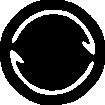
\includegraphics[height=0.4cm, keepaspectratio]{../!config/Bilder/bt_sync_logo.pdf} 
	{\large \textbf{Bittorrent} Sync} \\
	\texttt{B6WH2DISQ5QVYIRYIEZSF4ZR2IDVKPN3I}
	}
\end{minipage}
}


\begin{document}
\pagenumbering{Roman}
\maketitle
\begin{abstract}
\section*{Vorwort --- Mitarbeit am Skript}
Dieses Dokument ist eine Mitschrift aus der Vorlesung \enquote{\fach, \semester}, gelesen von \prof. Der Inhalt entspricht weitestgehend dem Tafelanschrieb. Für die
Korrektheit des Inhalts übernehme ich keinerlei Garantie! Für Bemerkungen und Korrekturen -- und seien es nur Rechtschreibfehler -- bin ich sehr dankbar. 
Korrekturen lassen sich prinzipiell auf drei Wegen einreichen: 
\begin{itemize}
	\item Persönliches Ansprechen in der Uni, Mails an \hrefsymmail{mailto:\mail}{\mail} (gerne auch mit annotieren PDFs) 
	\item \emph{Direktes} Mitarbeiten am Skript: Den Quellcode poste ich auf GitHub (siehe oben), also stehen vielfältige Möglichkeiten der Zusammenarbeit zur Verfügung:
	Zum Beispiel durch Kommentare am Code über die Website und die Kombination Fork + Pull Request. Wer sich verdient macht oder ein Skript zu einer Vorlesung, die 
	ich nicht besuche, beisteuern will, dem gewähre ich gerne auch Schreibzugriff.
	
	Beachten sollte man dabei, dass dazu ein Account bei \url{github.com} notwendig ist, der allerdings ohne Angabe von persönlichen Daten angelegt werden kann. 
	Wer bei GitHub (bzw. dem zugrunde liegenden Open-Source-Programm \enquote{\texttt{git}}) -- verständlicherweise -- Hilfe beim Einstieg braucht, dem helfe ich gerne 
	weiter. Es gibt aber auch zahlreiche empfehlenswerte Tutorials im Internet.\footnote{zB. \url{https://try.github.io/levels/1/challenges/1}, ist auf Englisch, aber dafür 
	interaktives LearningByDoing}
	\item \emph{Indirektes} Mitarbeiten: \TeX-Dateien per Mail verschicken. 
	
	Dies ist nur dann sinnvoll, wenn man einen ganzen Abschnitt ändern möchte (zB. einen alternativen Beweis geben), da ich die Änderungen dann per Hand einbauen muss! Ich freue mich aber auch über solche Beiträge!
\end{itemize}
\section*{Vorlesungshomepage}
{\centering 
\begin{minipage}[c][][c]{\textwidth}
	\centering \qrcode[height=3cm]{\homepage} \medskip\\
	\footnotesize \url{\homepage}
\end{minipage}
\par}

\end{abstract}

\tableofcontents
\cleardoubleoddemptypage

\pagenumbering{arabic}
\setcounter{page}{1}
\setcounter{footnote}{0}

\section{Kohomologie} % (fold)
\label{sec:1}

\begin{definition}[{name=[Kokettenkomplex und Kohomologie]}]
	Sei $R$ ein Ring. Ein \bet{$R$-Kokettenkomplex}\index{Kokettenkomplex} $(C^*,d^*)$ ist eine Folge von $R$-Moduln $(C^n)_{n \in \mathbb{N}}$ zusammen mit $R$-linearen Abbildungen 
	$d^n \colon C^n \to C^{n+1}$, sodass $d^{n+1} \circ d^n =0$ gilt. Der \bet{$n$-te Kohomologiemodul}\index{Kohomologiemodul} von $(C^*,d^*)$ ist definiert als 
	\[
		H^n(C^*,d^*) = \frac{\ker d^n \colon C^n \to C^{n+1}}{\im d^{n-1} \colon C^{n-1} \to C^n} 
	\]
	Sei $(D^*,d^{*})$ ein weiterer Kokettenkomplex.
	Eine \Index{Kokettenabbildung} ist eine Folge von $R$-linearen Abbildungen $f^n\colon C^n\to D^n$, sodass $ d^n_D \circ f^n = f^{n+1}\circ d^n_C$ für alle $n$ gilt. Ist 
	auch $g^n \colon C^n \to D^n$ eine Kokettenabbildung, so nennen wir eine $R$-lineare Abbildung $h^n \colon C^n \to D^{n-1}$ mit
	\[
		f^n - g^n  = h^{n+1} \circ d_C^n + d_D^{n-1} \circ h^n 
	\]
	eine \Index{Kokettenhomotopie} zwischen $f$ und $g$. Zu jeder Kokettenabbildung $f^n\colon C^n\to D^n$ gibt es eine 
	\bet{induzierte Abbildung}\index{induzierte Abbildung!Kohomologie} auf Kohomologie genau wie bei Homologie.
	
\end{definition}

\begin{bemerkung} \leavevmode
	\begin{enumerate}[i)]
		\item Sei $(C_*,d_*)$ ein $R$-Kettenkomplex und $V$ ein $R$-Modul. Dann erhalten wir einen $R$"=Kokettenkomplex $(C^*,d^*)$ durch 
		\[
			C^n \coloneqq \Hom_R(C_n,V) 
		\]
		und $d^n \colon C^n \to C^{n+1}$ definiert durch $\alpha \mapsto \alpha \circ d_{n+1}$. Dieser Kokettenkomplex $(C^*,d^*)$ heißt der 
		\bet{$V$-duale}\index{Kokettenkomplex!$V$-dualer Kokettenkomplex} Kokettenkomplex zu $(C_*,d_*)$. 
		\item Benutzen wir $\mathbb{Z}$ statt $\mathbb{N}$ als Indexmenge, so können wir durch $(C^n,d^n) \leadsto (C_n \coloneqq C^{-n}, d_n \coloneqq d^{-n})$ jeden Kokettenkomplex einem 
		Kettenkomplex zuordnen. Dieser Prozess ist offensichtlich umkehrbar.
	\end{enumerate}
\end{bemerkung}

\begin{beispiel}[{name=[Kohomologie ist nicht Dualisieren von Homologie]}]
	Es sei $(C_*,d_*)= \big(\begin{tikzcd}[cramped] \mathbb{Z} & \mathbb{Z} \lar["\cdot 2","d_1"'] & 0 \lar & \ldots \lar \end{tikzcd}\big)$ ein Kettenkomplex. 
	Dann ist
	\[
		H_k(C_*,d_*) = \begin{cases}
			\nicefrac{\mathbb{Z}}{2 \mathbb{Z}}, &\text{ falls } k =0\\
			0 , & \text{ sonst} 
		\end{cases}
	\]
	Der $\mathbb{Z}$-duale Kokettenkomplex hat dann folgende Gestalt
	\[
		\begin{tikzcd}
			 \Hom_{\mathbb{Z}}(\mathbb{Z},\mathbb{Z}) \rar["d^0"] \dar["\cong" description] & \Hom_{\mathbb{Z}}(\mathbb{Z},\mathbb{Z}) \rar \dar["\cong" description] 
			& 0 \rar & \ldots \\
			\mathbb{Z} \rar["\cdot 2"] & \mathbb{Z}
		\end{tikzcd}
	\]
	Damit ist die Kohomologie $H^k(C^*,d^*)=0$ für $k \neq 1$ und isomorph zu $\sfrac{\mathbb{Z}}{2 \mathbb{Z}}$ für $k=1$.
	Es gilt also nicht immer $H^*(\Hom(C_*;R),d^*) =  \Hom \enbrace{H_*(C_*,d_*),R}$. 
\end{beispiel}

\begin{definition}[{name=[singulärer Kokettenkomplex]}]
	Sei $(X,A)$ ein Paar von topologischen Räumen und $V$ eine abelsche Gruppe. Der \Index{singuläre Kokettenkomplex} von $(X,A)$ mit Koeffizienten in $V$ ist definiert durch
	\[
		C_\sing^*(X,A;V) \coloneqq \Hom_\mathbb{Z} \enbrace[\big]{C_*^\sing(X,A),V}
	\]
	und $d^*_\sing(\alpha) \coloneqq - (-1)^{\abs{\alpha}} \cdot \alpha \circ d_{*+1}^\sing$. Dabei ist $\abs{\alpha}=n$ für $\alpha \in C^n_\sing(X,A;R)$. Die 
	Kohomologie von $\enbrace[\big]{C^*_\sing(X,A;V), d^*_\sing}$ heißt die \Index{singuläre Kohomologie} von $(X,A)$ mit Koeffizienten in $R$.
\end{definition}

\begin{bemerkung}
	Sei $R$ ein kommutativer Ring und $V$ ein $R$-Modul. Dann ist
	\(
		\enbrace*{C^*_\sing(X,A;V), d^*_\sing}
	\)
	isomorph zum $V$-dualen $R$-Kokettenkomplex des $R$-Kettenkomplexes $\enbrace*{C^\sing_*(X,A;R), d^\sing_*}$.
\end{bemerkung}


\begin{definition}[{name=[induzierte Abbildung auf Kokettenkomplexen]}]
	Sei $f \colon (X,A) \to (Y,B)$ eine stetige Abbildung von Paaren. Dann erhalten wir eine Kokettenabbildung $f^* \colon C^*_\sing(Y,B;V) \to C^*_\sing(X,A;V)$ durch
	\index{induzierte Abbildung!singuläre Kokettenkomplexe}
	\[
		f^*(\alpha) \coloneqq \alpha \circ f_*
	\]
\end{definition}

\begin{bemerkung}
	Ist $g \colon (Y,B) \to (Z,C)$ eine weitere Abbildung von Paaren, so gilt $(g \circ f)^* = f^* \circ g^*$.
\end{bemerkung}

\begin{definition}[{name=[kontravarianter Funktor]}]
	Seien $\mathcal{C}$ und $\mathcal{D}$ Kategorien. Ein \Index{kontravarianter Funktor}  $F \colon \mathcal{C} \to \mathcal{D}$ ordnet jedem Objekt $C$ in $\mathcal{C}$ ein Objekt
	$D$ in $\mathcal{D}$ zu und jedem Morphismus $f \colon C \to C'$ einem Morphismus $F(f) \colon F(C') \to F(C)$ in $\mathcal{D}$ zu. Dabei muss gelten:
	\begin{enumerate}[i),noitemsep]
		\item $F(\id_C)= \id_{F(C)}$
		\item Für $\begin{tikzcd}[cramped] C \rar["f"] & C' \rar["f'"] & C'' \end{tikzcd}$ gilt $F(f' \circ f) = F(f) \circ F(f')$. 
	\end{enumerate}
	Kürzer ist ein \emph{kontravarianter} Funktor $F \colon \mathcal{C} \to \mathcal{D}$ das selbe wie ein \emph{kovarianter} Funktor 
	$\mathcal{C} \to \mathcal{D}^\op$.
\end{definition}

\begin{beispiel} Es gibt zahlreiche Beispiele für kontravariante Funktoren:
	\begin{enumerate}[i),itemsep=0pt]
		\item $\id \colon \mathcal{C} \to \mathcal{C}^\op$ ist kontravariant.
		\item Sei $V$ eine abelsche Gruppe. Wir erhalten einen kontravarianten Funktor
		\[
			\Hom(-,V) \colon \mathbb{Z}\text{-}\MOD  \longrightarrow \mathbb{Z}\text{-}\MOD
		\]
		\item Sei $V$ eine abelsche Gruppe. Dann sind 
		\begin{align}
			C_\sing^*(-,V) &\colon \TOP^2 \longrightarrow \mathbb{Z}\text{-}\textsc{Kokettenkomplexe}  \\
			H^*_\sing \enbrace[\big]{C_\sing^*(-,V),d_\sing^*} &\colon \TOP^2 \longrightarrow \textsc{Gr}\text{-}\mathbb{Z}\text{-}\MOD   
		\end{align}
		kontravariante Funktoren.
	\end{enumerate}
\end{beispiel}

\begin{satz}[{name=[Eigenschaften singulärer Kohomologie]}]
	Singuläre Kohomologie hat die folgenden Eigenschaften:
	\begin{enumerate}[i),itemsep=1.5pt]
		\item \textbf{Dimensionsaxiom:} Es gilt $H^n_\sing(\set{\pt};V) = V$, falls $n=0$ ist und sonst $0$.\index{Dimensionsaxiom} 
		\item \textbf{Paarfolge:} Es gibt eine natürliche Transformation $\partial^*\colon H^*(A;V) \to H^{*+1}(X,A;V)$ sodass für jedes Paar\index{Paarfolge} 
		\[
			\begin{tikzcd}
				0 \rar & H^0(X,A;V) \rar & H^0(X,V) \rar & H^0(A;V) \rar["\partial"] & H^1(X,A;V) \rar & \ldots 
			\end{tikzcd}
		\]
		eine lange exakte Folge ist. $\partial$ bezeichnet man auch als \Index{verbindende Abbildung}.
		\item \textbf{Ausschneidung:} Sei $L \subseteq A$ mit $\overline{L} \subseteq \mathring{A}$. Dann induziert die Inklusion \index{Ausschneidung}
		$i \colon (X \setminus L, A \setminus L) \hookrightarrow (X,A)$ einen Isomorphismus $i^* \colon H^*(X,A;V) \to H^*(X \setminus L, A \setminus L;V)$.
		\item \textbf{Homotopieinvarianz:} Sind $f,g \colon (X,A) \to (Y,B)$ homotope Abbildungen von Paaren, so gilt $f^* = g^*$ für die induzierten Abbildungen in singulärer 
		Kohomologie.\index{Homotopieinvarianz}
	\end{enumerate}
\end{satz}
\begin{beweis}
	Für singuläre Homologie haben wir die entsprechenden Aussagen schon bewiesen. In allen vier Fällen folgt die Aussage für Kohomologie aus schon bewiesenen Aussagen über 
	den singulären Kettenkomplex.\todo{Andere Teile aus Übungen übernehmen}
	
	Wir führen dies an dieser Stelle nur für iv) aus. Seien $f, g \colon X \to Y$ homotop. Dann gibt es eine Kettenhomotopie $H \colon C^\sing_*(X) \to C^\sing_{*+1}(Y)$ zwischen den 
	auf dem singulären Kettenkomplex induzierten Abbildungen $f_*$ und $g_*$. Es gilt also
	\[
		d_{n+1} \circ H + H \circ d_n = f_* - g_*
	\]
	$H$ induziert $H^\# \colon C^*_\sing(Y;V) \to C_\sing^{*-1}(X;V)$ mit $H^\#(\alpha) \coloneqq (-1)^{\abs{\alpha}} \cdot \alpha \circ H$. Es gilt nun für $\alpha \in C_\sing^n(Y;V)$
	\begin{align}
		\enbrace*{d^{n-1} \circ H^\# + H^\# \circ d^n}(\alpha) &= d^{n-1} \circ H^\#(\alpha) + H^\# \circ d^n (\alpha)\\
		&= d^{n-1} \enbrace[\big]{(-1)^n \cdot (\alpha \circ H)} - (-1)^n \cdot H^\# \enbrace*{\alpha \circ d_{n+1}} \\
		&= (-1)^n \cdot \enbrace*{(-1)^{n} \alpha \circ H  \circ d_n - (-1)^{n+1} \alpha \circ d_{n+1} \circ H} \\
		&= \alpha \circ H \circ d_n + \alpha \circ d_{n+1} \circ H \\
		&= \alpha \enbrace*{f_* - g_*} = f^*(\alpha) - g^*(\alpha) 
	\end{align}
	Damit ist $f^* - g^* =0$ in Kohomologie, da die linke Seite für $\alpha \in \ker d^n$ im Bild von $d^{n-1}$ liegt. \todo{Revision}
\end{beweis}

\begin{bemerkung}[{name=[Angabe des Verbindungshomomorphismus]}]
	Sei $(X,A)$ ein Paar von topologischen Räumen. Der Verbindungshomomorphismus $\partial \colon H^n(A;V) \to H^{n+1}(X,A;V)$ kann wie folgt beschrieben werden: Sei 
	$\alpha \colon C_n(A) \to V$ ein Kozykel. Setze $\alpha$ zu $\hat{\alpha} \colon C_n(X) \to V$ fort. Dann ist \marginnote{Da muss ich nochmal drüber nachdenken…}
	\[
		\partial \benbrace{\alpha} = \benbrace*{d^n \hat{\alpha}} \in H^{n+1}(X,A;V)
	\]
\end{bemerkung}

\begin{beispiel}
	Die Gruppe $H^0(X;V)$ ist die Gruppe aller Abbildungen $\xi \colon X \to V$, die konstant auf Wegzusammenhangskomponenten ist. Die Gruppe $H^0(X,A;V)$ besteht aus allen 
	solchen Abbildungen, die zusätzlich auf $A$ trivial sind.
\end{beispiel}

\begin{definition}[{name=[Produkt von $R$-Moduln]}]
	Seien $(V_i)_{i \in I}$ $R$-Moduln. Mit $V \coloneqq \prod_{i \in I} V_i$ bezeichnen wir das \Index{Produkt} der $V_i$. Element in $V$ sind $I$-Folgen $(v_i)_{i \in I}$ mit 
	$v_i \in V_i$. Die $R$-Modulstruktur ist erklärt durch
	\begin{align}
		(v_i)_{i \in I}+ (w_i)_{i \in I} &\coloneqq (v_i + w_i)_{i \in I} \\
		r \cdot (v_i)_{i \in I} & \coloneqq (r \cdot v_i)_{i \in I}
	\end{align}
	Für jedes $i_0 \in I$ erhalten wir $\pi_{i_0} \colon V \to V_{i_0}$, $(v_i)_{i \in I} \mapsto v_{i_0}$
\end{definition}

\begin{bemerkung}[name={Universelle Eigenschaft des Produktes}]
	Seien $V_i$, $i \in I$ $R$-Moduln. Sei $W$ ein weiterer $R$-Modul. Dann gibt es zu jeder Folge $(f_i \colon W \to V_i)_{i \in I}$ von $R$-linearen Abbildungen eine eindeutige 
	$R$-lineare Abbildung $f \colon W \to \prod_{i \in I}V_i$ mit $f_i= \pi_i \circ f$. Diese ist gegeben durch
	$f(w) \coloneqq \enbrace*{f_i(w)}_{i \in I}$.
\end{bemerkung}

\begin{bemerkung}
	Ist $I$ endlich, so gilt
	\[
		\bigoplus_{i \in I} V_i = \prod_{i \in I} V_i
	\]
\end{bemerkung}

\begin{bemerkung}
	Es seien $V_i$, $i \in I$ $R$-Moduln. Sei $W$ ein weiterer $R$-Modul. Seien $j_{i_0} \colon V_{i_0} \to \bigoplus_{i \in I}V_i$ die Inklusionen $v_{i_0} \mapsto (v_i)_{i \in I}$
	mit $v_i =v_{i_0}$ für $i=i_0$ und $0$ sonst. Dann erhalten wir einen Isomorphismus
	\mapdef{\Hom_R \enbrace[\big]{\bigoplus_i V_i,W}}{\prod_{i \in I} \Hom_R(V_i,W)}{f}{(f \circ j_i)_{i \in I}}{\cong}
\end{bemerkung}

\begin{satz}
	Sei $X= \coprod_{i \in I} X_i$ die Summe von topologischen Räumen $X_i$. Dann induzieren die Inklusionen $j_i \colon X_i \to X$ einen Isomorphismus 
	\[
		\begin{tikzcd}[row sep=0em]
			H^* \enbrace*{X,V} \rar & \prod_{i \in I} H^*(X_i,V) \\
			\xi \rar[mapsto] & \enbrace[\big]{(j_i)^*(\xi)}_{i \in I}
		\end{tikzcd}
	\]
\end{satz}
\begin{beweis}
	Die $(j_i)_{i \in I}$ induzieren einen Isomorphismus von Kettenkomplexen $\varphi \colon \bigoplus_{i \in I}C_*(X_i) \to C_*(X)$,  
	$(a_i)_{i \in I} \mapsto \sum_{i \in I} (j_i)_* (a_i)$. Wegen 
	\[
		\Hom \enbrace*{\bigoplus\nolimits_{i \in I} C_*(X_i),V} = \prod_{i \in I} \Hom \enbrace*{C_*(X_i),V}
	\]
	erhalten wir einen Isomorphismus von Kokettenkomplexen
	\[
		\begin{tikzcd}[row sep=0em]
			C^*(X,V) \rar["\cong"] & \prod_{i \in I} C^*(X_i,V) \\
			\alpha \rar[mapsto] & \enbrace[\big]{j_i^*(\alpha)}_{i \in I}
		\end{tikzcd}
	\]
	Dieser induziert den behaupteten Isomorphismus in Kohomologie.  
\end{beweis}

\begin{definition}[{name=[reduzierte Kohomologie]}]
	Die reduzierte Kohomologie von $X$, $\tilde{H}^*(X;V)$ ist definiert als der Kokern von $p^* \colon H^* \enbrace*{\set{\pt};V} \to H^*(X;V)$.
\end{definition}

\begin{bemerkung}[{name=[Zusammenhang zwischen reduzierter und regulärer Homologie]}]
	Für reduzierte Kohomologie gilt
	\[
		H^n(X;V) \cong \begin{cases}
			\tilde{H}^n(X;V), &\text{ falls } n \not= 0\\
			\tilde{H}^0(X;V) \oplus V , &\text{ falls } n=0 
		\end{cases}
	\]
\end{bemerkung}

\begin{beispiel}[{name=[Kohomologie der Sphäre]}]
	Die reduzierte Kohomologie der Sphäre ist gegeben durch
	\[
		\tilde{H}^l (S^n;V) \cong H^l \enbrace*{D^n,S^{n-1};V} \cong \begin{cases}
			V, &\text{ falls } l=n\\
			0, &\text{ sonst}  
		\end{cases}
	\]
\end{beispiel}
% section 1 (end)
\newpage

\section{Die Paarung zwischen Kohomologie und Homologie} % (fold)
\label{sec:2}

\begin{definition}[{name=[Paarung]}]
	Sei $V$ ein $\mathbb{Z}$-Modul, $(X,A)$ ein Paar von topologischen Räumen. Wir definieren die \Index{Paarung}
	\[
		\begin{tikzcd}[row sep=0cm]
			H^n(X,A;V) \times H_n(X,A) \rar & V \\
			(\xi, x) \rar[mapsto] & \xi(x)
		\end{tikzcd}
	\]
	wie folgt: Wähle $\alpha \in C^n_\sing(X,A;V)$ mit $\benbrace*{\alpha}=\xi$ und $a \in C^\sing_n(X,A)$ mit $\benbrace*{a}=x$. Dann setze $\xi(x) \coloneqq \alpha(a)$.
\end{definition}

\begin{bemerkung}
	Sei $\beta \in C^{n-1}_\sing(X,A;V)$ und $b \in C^\sing_{n+1}(X,A)$. Dann 
	\begin{align}
		\enbrace*{\alpha + d^{n-1}(\beta)}(a + d_{n+1}(b)) = \alpha(a) + \Underbrace{\alpha \enbrace[\big]{d_{n+1}(b)}}{=0 \text{ da } d^n \alpha=0 } + \Underbrace{d^{n-1}(\beta) \enbrace*{a + d_{n+1}(b)}}{\pm \beta \enbrace[\big]{d_n(a + d_{n+1}(b))}} 
	\end{align}
\end{bemerkung}

\begin{bemerkung}
	Für $r \in \mathbb{Z}$, $x,x' \in H_n(X,A)$, $\xi,\xi' \in H^n(X,A;V)$ gilt
	\begin{align}
		(r \cdot \xi)(x) &= r \cdot \xi(x) = \xi(r \cdot x) \\
		(\xi +\xi')(x) &= \xi(x) + \xi'(x) \\
		\xi(x+x')&= \xi(x) + \xi(x')
	\end{align}
\end{bemerkung}

\begin{bemerkung}
	Wir können $(\xi,x)\mapsto \xi(x)$ auch als interpretieren als Homomorphismus
	\[
		f \colon H^n(X,A;V) \longrightarrow \Hom_\mathbb{Z} \enbrace[\big]{H_n(X,A),V}
	\]
	mit $f(\xi)= \enbrace*{x \mapsto \xi(x)}$.
\end{bemerkung}

\begin{satz}[label=eig_kohomo_to_hom_homo]
	Für die eben definierte Abbildung $f \colon H^n(X,A;V) \to \Hom_\mathbb{Z} \enbrace[\big]{H_n(X,A),V}$ gilt
	\begin{enumerate}[(i)]
		\item $f$ ist surjektiv
		\item Ist $V$ ein $\mathbb{Q}$-Vektorraum, so ist $f$ auch injektiv.
	\end{enumerate}
\end{satz}

Um den Satz beweisen zu können, benötigen wir zunächst zwei technische Aussagen:

\begin{lemma}[label=lem:untergrp_frei]
	Untergruppen freier abelscher Gruppen sind frei.
	% Sei $C$ eine Untergruppe der freien abelschen Gruppe $\mathbb{Z}[S]$. Dann gibt es $T \subseteq S$ und eine $T$-Folge $(n_t)_{t \in T}$ von positiven Zahlen $n_t$, so dass $C$
	% das Bild der injektiven Abbildung $M \colon \mathbb{Z}[T] \to \mathbb{Z}[S]$, $\sum z_t t \mapsto \sum z_t m_t \cdot t$ ist. Insbesondere ist $C$ frei.
\end{lemma}
\begin{beweis}
	Sei $C$ eine Untergruppe von $\mathbb{Z}[S]$. Sei $\mathcal{M}$ die Menge der Tripel $(T,R,\varphi)$ mit
	\begin{itemize}
		\item $T \subseteq R \subseteq S$.
		\item $\varphi \colon \mathbb{Z}[T] \to \mathbb{Z}[R] \cap C$ ein Isomorphismus.
	\end{itemize}
	Wir definieren eine partielle Ordnung auf $\mathcal{M}$ durch
	\[
		(T,R,\varphi) \le (T',R',\varphi') :\iff T \subseteq T', R \subseteq R', \varphi'|_{T}=\varphi
	\]
	Das Lemma von Zorn liefert uns die Existenz eines maximalen Elements $(T,R,\varphi) \in \mathcal{M}$. Zu zeigen bleibt $R=S$. Angenommen es existiert ein $s \in S \setminus R$.
	Ist $C \cap \mathbb{Z}[R \cup \set{s}] = C \cap \mathbb{Z}[R]$, so ist $(T,R,\varphi) \lneqq (T,R \cup \set{s},\varphi) \in \mathcal{M}$ im Widerspruch zur Maximalität von 
	$(T,R,\varphi)$. Sei also $\mathbb{Z}[R] \cap C \subsetneq \mathbb{Z}[R \cup \set{s}] \cap C$. Betrachte die kurze exakte Sequenz \todo{Diagramm vervollständigen}
	\[
		\begin{tikzcd}
			\mathbb{Z}[R] \cap C \rar[hook] \dar[hook,"i_0"]& \mathbb{Z}[R \cup \set{s}] \cap C \rar[two heads] \dar[hook,"i_1"] & \sfrac{\mathbb{Z}[R \cup \set{s}] \cap C}{\mathbb{Z}[R] \cap C} 
			\dar["i_2"] \\
			\mathbb{Z}[R] \rar[hook] & \mathbb{Z}\benbrace*{R \cup \set{s}} \rar[two heads,"p"] & \mathbb{Z}\benbrace*{\set{s}}
		\end{tikzcd}
	\]
	Nun ist $\mathbb{Z}[R] \cap C  = (\mathbb{Z}[R]) \cap \enbrace*{\mathbb{Z}[R \cup \set{s}] \cap C}$. Damit muss dann die von $i_0$ und $i_1$ induzierte Abbildung 
	$i_2 \colon \sfrac{\mathbb{Z}[R \cup \set{s}] \cap C}{\mathbb{Z}[R] \cap C} \to \mathbb{Z}[\set{s}]$ injektiv sein. Es folgt, dass $\im i_2 = \mathbb{Z}\benbrace*{\set{m \cdot s}}$
	ist für ein $m >0$. Sei $c \in \mathbb{Z}[R \cup \set{s}] \cap C$ ein Urbild von $m \cdot s$ unter $p \circ i_1$. Nun können wir $\varphi$ durch $s \mapsto c$ zu
	$\varphi^+ \colon \mathbb{Z}\benbrace*{T \cup \set{s}} \to \mathbb{Z}\benbrace*{R \cup \set{s}} \cap C$. Es folgt, dass $\varphi^+$ ein Isomorphismus ist im Widerspruch zur 
	Maximalität von $(T,R,\varphi)$.
	% Sei $\mathcal{M}$ die Menge aller Tripel $(T,R,m)$ mit
	% \begin{itemize}
	% 	\item $T \subseteq R \subseteq S$
	% 	\item $m=(m_t)_{t \in T}$ ist eine $T$-Folge von positiven Zahlen
	% 	\item das Bild von $M \colon \mathbb{Z}[T] \to \mathbb{Z}[S]$, $t \mapsto m_t \cdot t$ ist $C \cap \mathbb{Z}[R]$.
	% \end{itemize}
	% Wir definieren eine partielle Ordnung auf $\mathcal{M}$ durch
	% \[
	% 	(T,R,m) \le (T',R',m') :\iff T \subseteq T', R \subseteq R', m'|_{T}=m
	% \]
	% Es ist $\mathcal{M} \not= \emptyset$, da $(\emptyset,\emptyset, \cdot ) \in \mathcal{M}$. Jede aufsteigende Ketten in $\mathcal{M}$ hat eine obere Schranke. Nach Zorns Lemma
	% existiert ein maximales Element $(T,R,m) \in \mathcal{M}$. Es bleibt zu zeigen: $R=S$.
\end{beweis}

\begin{lemma}[label=lem:abel_qvek]
	Sei $A_0$ eine Untergruppe der abelschen Gruppe $A$, $V$ ein $\mathbb{Q}$-Vektorraum und $\beta_0 \colon A_0 \to V$ ein Gruppenhomomorphismus. Dann gibt es eine Fortsetzung 
	$\beta \colon A \to V$ von $\beta_0$ zu einem Gruppenhomomorphismus.  
\end{lemma}
\begin{beweis}
	Die Inklusion $i \colon A_0 \to A$ induziert einen injektiven\footnote{nach Übungsaufgabe} $\mathbb{Q}$-Vektorraum-Homomorphismus 
	\[
		\mathbb{Q}\otimes i \colon \mathbb{Q} \otimes A_0 \longrightarrow \mathbb{Q} \otimes A , \qquad q \otimes a_0 \mapsto q \otimes i(a_0)
	\]
	Nun können wir die $\mathbb{Q}$-lineare Abbildung $q \otimes a_0 \mapsto q \cdot \beta_0(a_0) \in V$ von $\mathbb{Q} \otimes A_0$ zu 
	$\overline{\beta} \colon \mathbb{Q} \otimes A \to V$ fortsetzen. Dann ist $a \mapsto \overline{\beta}(1 \otimes a)$ die gesuchte Fortsetzung von $\beta_0$.
\end{beweis}

\begin{beweis}[name={von \autoref{eig_kohomo_to_hom_homo}}] \leavevmode
	\begin{enumerate}[(i)]
		\item Sei $\varphi \colon H_n(X,A) \to V$ gegeben. Sei $p \colon\ker d_n \twoheadrightarrow H_n(X,A)$ die Projektion. Betrachte die kurze exakte Folge 
	\[
		\begin{tikzcd}
			\ker  d_n \rar[hook,"i"] & C_n^\sing(X,A) \rar["d_n",two heads] & \im d_n
		\end{tikzcd}
	\]
	Als Untermodul des freien Moduls $C_{n-1}^\sing(X,A)$ ist nach \autoref{lem:untergrp_frei} $\im d_n$ frei, insbesondere spaltet die kurze exakte Sequenz, insbesondere ist
	$C^\sing_n(X,A) \cong \ker d_n \oplus \im d_n$. Daher können wir $\varphi \circ p \colon \ker d_n \to V$ zu $\alpha \colon C_n^\sing(X,A) \to V$ fortsetzen. Genauer: Sei 
	$s \colon \im d_n \to C_n^\sing(X,A)$ ein Spalt. Dann können wir $\alpha \colon C_n^\sing(X,A) \to V$ definieren durch 
	\[
		\alpha(a) \coloneqq \varphi \circ p \enbrace*{a - s \enbrace[\big]{d_n(a)}}
	\]
	Es folgt $d_n \circ \alpha =0$ und $f \enbrace*{[\alpha]}=\varphi$.
	\item Sei $\alpha \in C^n_\sing(X,A;V)$ mit $d^n(\alpha)=0$. Sei $\benbrace*{\alpha} \in \ker f$, also $\alpha(a)=0$ für alle $a \in \ker d_n$.  Dann faktorisiert $\alpha$ über
	$\im d_n \subseteq C_{n-1}(X,A)$: $\alpha$ induziert $\beta_0 \colon \im d_n \to V$ mit $\alpha = \beta_0 \circ d_n$. Ist $V$ ein $\mathbb{Q}$-Vektorraum, so können wir 
	$\beta_0$ nach \autoref{lem:abel_qvek} zu $\beta \colon C_{n-1}(X,A) \to V$ fortsetzen. Es folgt 
	$\benbrace*{\alpha}= \benbrace*{\beta \circ d_n} = \pm \enbrace*{d^{n+1} \beta}=0$. \qedhere
	\end{enumerate}
\end{beweis}

\begin{korollarB}
	Es gilt $H^n(X,A;\mathbb{Q}) \cong \Hom \enbrace*{H_n(X,A);\mathbb{Q}}$
\end{korollarB}

\begin{bemerkung}
	Es gilt sogar $H^n \enbrace*{X,A;\mathbb{Q}} \cong \Hom_\mathbb{Q} \enbrace*{H_n(X,A;\mathbb{Q}),\mathbb{Q}}$.
\end{bemerkung}
\newpage
% section 2 (end)

\section{Produkte auf Kohomologie} % (fold)
\label{sec:3}

\begin{definition}
	Sei $\sigma \colon \abs{\Delta^n}  \to X$ ein singulärer Simplex in $X$. Für $0 \le p \le n$ definieren wir
	\[
		\sigma|_{\benbrace*{0,\ldots ,p}} \colon \abs{\Delta^p} \to X \quad , \quad \sigma|_{\benbrace{p,\ldots ,n}} \colon \abs{\Delta^{n-p} \to X}  
	\]
	durch $\sigma|_{\benbrace*{0,\ldots ,p}}(t_0, \ldots ,p) = \sigma \enbrace*{t_0, \ldots , t_p, 0, \ldots ,0}$ und 
	$\sigma|_{p,\ldots ,n}(t_{p}, \ldots ,t_n)= \sigma(0,\ldots ,0,t_{p}, \ldots , t_n)$
\end{definition}

\begin{bemerkung}
	Wir schreiben auch $\sigma|_{\benbrace*{0,\ldots , \not i, \ldots ,n}}$ für die $i$-te Seite von $\sigma$.
\end{bemerkung}

\begin{definition}
	Sei $R$ ein Ring und $A,B \subseteq X$. Wir definieren das \Index{$\cup$-Produkt} auf dem singulären Kokettenkomplex 
	\[
		\cup \colon C^p_\sing \enbrace*{X,A;R} \otimes C^q_\sing(X,B;R) \longrightarrow C^{p+q}_\sing \enbrace*{X,A \cup B;R}
	\]
	durch $(\alpha \cup \beta)(\sigma) \coloneqq  (-1)^{p \cdot q} \cdot \alpha\enbrace*{\sigma|_{\benbrace{0,\ldots ,p}}} \cdot \beta \enbrace*{\sigma|_{\benbrace*{p, \ldots , p+q}}}$.
\end{definition}

\noindent\todo[inline]{Zeichnung für $n=2$ einfügen}

\begin{lemma}\leavevmode
	\begin{enumerate}[1)]
		\item $d^{p+q}(\alpha \cup \beta) = d^p(\alpha) \cup \beta + (-1)^p \cdot \alpha \cup d^q(\beta)$
		\item Das $\cup$-Produkt ist assoziativ.
		\item Für $f \colon X \to X'$ mit $f(A) \subseteq A'$, $f(B) \subseteq B'$ gilt $f^*(\alpha \cup \beta)= f^*(\alpha) \cup f^*(\beta)$ für $\alpha \in C^p_\sing(X',A';R)$, 
		$\beta \in C^q_\sing(X',B';R)$.
		\item Sei $1_X \in C_\sing^0(X;R)$ mit $1_X(\sigma)=1_R$ für alle $\sigma \colon \abs{\Delta^0} \to X$. Dann gilt $1_X \cup \alpha = \alpha = \alpha\cup 1_X$.
	\end{enumerate}
\end{lemma}
\begin{beweis}
	Übung bzw. Notizen auf Homepage \todo{\TeX{}en wenn Zeit}
\end{beweis}

\begin{definition}
	Die vom $\cup$-Produkt auf dem singulären Kokettenkomplex induzierte Abbildung in Kohomologie 
	\[
		\cup \colon H^p(X,A;R) \otimes H^q(X,B;R) \longrightarrow H^{p+q}(X,A;R)
	\]
	ist das $\cup$-Produkt in Kohomologie. $\benbrace*{\alpha} \cup \benbrace*{\beta} = \benbrace*{\alpha \cup \beta}$.
\end{definition}


% section 3 (end)









\cleardoubleoddemptypage
\pagenumbering{Alph}
\setcounter{page}{1}

\printindex
\listoffigures
\todototoc
\listoftodos[To-do's und andere Baustellen]
\end{document}
